%%%%%%%%%%%%%%%%%%%%%%%%%%%%%%%%%%%%%%%%%%%%%%%%%%%%%%%%%%%%%%%%%%%%
% Einleitung
%%%%%%%%%%%%%%%%%%%%%%%%%%%%%%%%%%%%%%%%%%%%%%%%%%%%%%%%%%%%%%%%%%%%

\chapter{Introduction}
\label{introduction}
While understanding the human body has provided many i.a. medical advancements, research mostly also reveals unknown facts and connections. As experimental methods advanced, many observed phenomenons could be linked to molecular-scale mechanisms. With new generation DNA sequencing, for example genetic diseases and their exact origin could be identified. While for illnesses like BSE a linkage to misfolded proteins was found, other illnesses like Alzheimer disease, which is also possibly connected to misfolded proteins, lack general treatment and a definite cause as of now~\cite{Burns2009}. This shows the need for further research and understanding of proteins in biological systems.\\
Proteomics is the interdisciplinary research field analyzing the composition, interaction and impacts of the proteome (the entirety of proteins) of single cells or up to a whole organism~\cite{Han2008, Sachsenberg2017}. It has grown in importance to the scientific community over the last decade due to new and refined methods enabling large-scale data acquisition, resulting in the publication of the first human proteome drafts in 2014~\cite{Wilhelm2014, Kim2014}. Meanwhile, methods of equally high quality are often missing for the study of many interactions with other (bio-)molecules. In this thesis, research was done to fit one piece of the data acquisition pipeline, the well established Percolator algorithm~\cite{Granholm2012}, onto the characteristics of protein-RNA interaction. We will focus on the research to this field based on the study of proteins cross-linked onto RNA.\\
The scientific background is covered in~\autoref{background}. Chapters~\ref{matmet} and~\ref{results} describe the changes done to the Percolator algorithm and their impact. Alongside an outlook for further possible improvements and experiments, these will be discussed in~\autoref{discussion}, concluding this thesis.

\section{Background}
\label{background}
	\subsection{Cross-linking}
	\label{lab:background:cross-linking}
	Cross-linking is the process of artificially inducing a chemical bond between different molecules, using for example UV light~\cite{Sachsenberg2017}. The hope of applying this to peptides and RNA, is to receive insight into their \textit{in~vivo} interactions, and possibly also conclusions about protein-DNA interaction.\\
	\subsection{Mass Spectrometry}
	\label{lab:background:ms}
	For quantitatively characterizing the proteome of a sample, large scale measuring techniques are needed. Mostly, mass spectrometry (MS) is used, or more specifically, as for the data in this thesis, tandem mass spectrometry (MS/MS) combined with liquid chromatography (LC). In order to analyze the protein sample with MS, its complexity has to be reduced as much as possible, for example using LC~\cite{Sachsenberg2017}. As~\citet{Han2008} explains, the mass spectrometer then produces mass spectra, which have to be analyzed further. It does so by first ionizing the substrate, because it can only detect charged particles. Then, the sample is separated in the mass analyzer by the ratio $\frac{m}{z}$, mass of the particles to their charge. The detector then quantifies the amount of a particle in the sample. The result is a mass spectrum, as shown in figure~\ref{fig:mass_spectrum}.\\
	\renewcommand{\baselinestretch}{0.9}
	\begin{figure}
		\normalsize
		\centering
		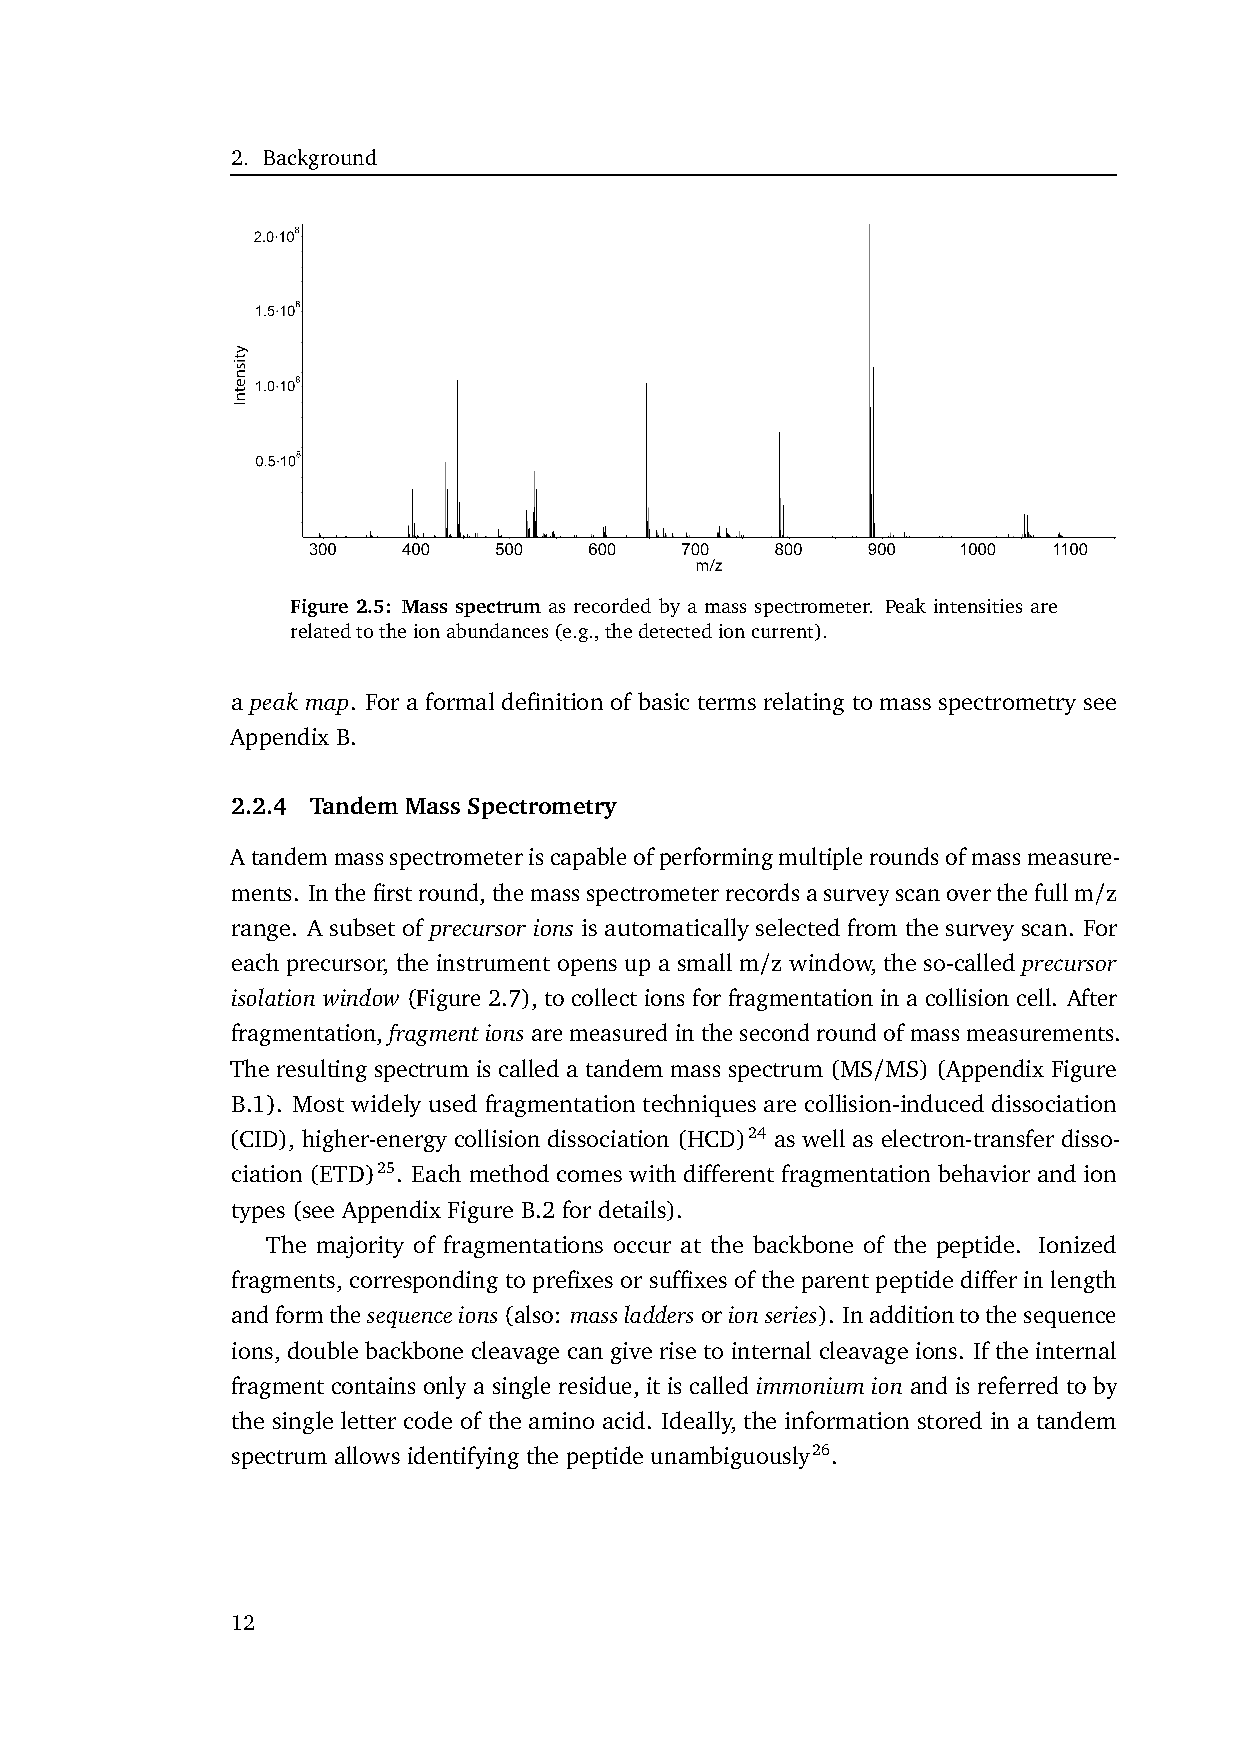
\includegraphics[width = \textwidth, trim=3.9cm 20cm 2.5cm 3cm,clip]{figures/Grafik_Timo.pdf}
		\caption[Example for a mass spectrum]{Example for a mass spectrum as recorded by a mass spectrometer. The ion intensity correlates with the amount of a molecule in the sample, $\frac{m}{z}$ is the mass-to-charge-ratio. From:~\citet{Sachsenberg2017}}
		\label{fig:mass_spectrum}
	\end{figure}
	\renewcommand{\baselinestretch}{1}
	Because mass alone does not give enough information about a peptide to determine its sequence, tandem mass spectrometry is often used to gather more detailed evidence. In this procedure, particles of similar $\frac{m}{z}$ ratio are selected for fragmentation in a collision cell after the first round of mass measurement~\cite{Sachsenberg2017}. In there, the substance collides with a gas to be broken down into smaller molecules. For proteins, fragmentation happens predominantly in their backbone, producing all possible sub-sequences of the peptide. This yields a spectrum that is almost unique for its protein, which allows for peptide identification using bioinformatics tools~\cite{Angel2012}.\\
	\subsection{Bioinformatics Tool}
	\label{lab:background:bioinfo_tools}
	Algorithms like Sequest~\cite{Eng1994} or X!~Tandem~\cite{Craig2004} compare the resulting spectra with theoretical spectra calculated from a list of possible peptides and compute a score based on their similarity. The peptides are generated by obtaining a list of proteins expected in the sample and calculating the peptides resulting from the, for example enzyme-based, degradation of the proteins. The best scoring peptide is then considered a peptide-spectrum-match (PSM). The scores produced by those algorithms often do not distinguish well enough between correct and incorrect matches~\cite{Kll2007}, but they enable FDR estimation using decoy databases and serve as a basis for score re-calibration with the Percolator~algorithm~\cite{Kll2007, Granholm2012}.\\
	Decoy databases are created from the target database, contain usually as  many peptides~\cite{Peng2003, Moore2002} in a reversed or shuffled order with respect to the amino acid sequence~\cite{Aggarwal2016}. They are presented to the scoring algorithm either separately~\cite{Granholm2012} or mixed with the target database~\cite{Peng2003}. It is assumed, that decoy and target peptides have similar features~\cite{Moore2002} and are not easily distinguishable by a scoring algorithm. When the actually fitting peptide for a given spectrum is not in the target database, and thus a wrong one will be chosen, the best scoring peptide will be a decoy approximately half of the time. This allows for an estimation of wrongly assigned targets, since the score distribution is assumed to be the same for decoys and false targets~\cite{Aggarwal2016}.\\
	In practice, one estimates the probability of a PSM being a false target by counting the number of decoy-PSMs with the same or a higher score. It is then assumed, there are as many false targets and thus a false discovery rate (FDR) can be estimated~\cite{Granholm2012}. This leads to the following formula\footnote{In this thesis, the following approximation is used:\\
		$FDR \approx \frac{\text{\# decoy PSMs}}{\text{\# all PSMs}} = \frac{\text{\# decoy PSMs}}{\text{\# decoy PSMs} + \text{\# target PSMs}}$\\
		It is faster to calculate and yields results differing by the FDR, so in the relevant range of FDRs of $0$ to $5\%$ up to $5\%$:\\
		$\frac{\frac{\text{\# decoys}}{\text{\# targets}}}{\frac{\text{\# decoys}}{\text{\# decoys} + \text{\# targets}}} = \frac{\text{\# decoys} + \text{\# targets}}{\text{\# targets}} = 1 + \frac{\text{\# decoys}}{\text{\# targets}} \approx 1 + FDR$\\}:
	\begin{equation}
	FDR = \frac{\text{\# false target PSMs}}{\text{\# all target PSMs}} \approx  \frac{\text{\# decoy PSMs}}{\text{\# all target PSMs}}
	\end{equation}
	The q-value as a measure for a single PSM rather than a metric for a set of PSMs is then derived from this as the minimum FDR of all PSMs with a lower or equal score~\cite{Granholm2012, Aggarwal2016}. It will be used for estimating the credibility for any one PSM.\\
	\subsection{Percolator}
	\label{lab:background:percolator} As \citet{Kll2007} say, separating correct from incorrect target PSMs with already mentioned algorithms works fine, but there is still room for improvement. This is because often not all information is used and considered jointly. Percolator~\cite{Kll2007, Granholm2012} tries to utilize as much information as possible by using scores from different algorithms, features of the peptide (like its length), of the spectrum, or the PSM itself. It joins them using a linear support vector machine (SVM) and a semi-supervised approach with cross-validation to retain as many PSMs as possible. In every iteration, the top ranking, non-decoy PSMs up to a certain threshold of q-value are chosen as positive training examples, and the decoy PSMs are used as negative training set. The PSMs are then re-ranked using the SVMs score with the intention of getting a better separation of true and false PSMs. If this holds true, the positive training set of the next iteration better is of higher quality and the SVM can be trained even better. The algorithm usually converges within the first 10 iterations~\cite{Kll2007}.\\
	As explained by~\citet{Bishop2006}, an SVM is a maximum margin classifier model. In the linear case, it tries to generate a hyperplane inside the multi-dimensional space that splits the given training data into the specified classes. For generalization performance, it tries to maximize the distance or margin between the hyperplane and the nearest training points, called support vectors. If the data is not linearly separable, it allows but punishes outliers by their distance to the hyperplane: An outlier inside the margin but on the correct side of the hyperplane is not penalized as badly as if it was on the wrong side of the hyperplane, and the further away from the hyperplane a point lies on the wrong side, the more this gets penalized. The strength of the penalization is also controlled by the parameter C, which can also be defined differently for points of different classes\footnote{https://scikit-learn.org/stable/modules/generated/sklearn.svm.LinearSVC.html}.\\
	To avoid having to split the data into training and testing set and consequently losing possibly correct PSMs but also avoid overfitting, a nested cross-validation approach is being used. As~\citet{Granholm2012} explain, overfitting is a central problem in machine learning. It happens when the model fits itself onto random variation in the data, not actually connected to a general pattern and performing poorly when presented new data. Cross-validation means splitting the data into a number smaller batches (Percolator uses $3$), presenting all but one to the model as training and the remaining part to validate the results, or, in the case of Percolator, to score the PSMs. For every part of the data a new model is trained by every part but the one to be scored, and the scores of different parts are normalized in the end. Additionally, Percolator performs cross-validation with every training batch, evaluating different parameters for the machine learning model applied to this specific batch of data~\cite{Granholm2012}.\\
	\subsection{ROC curves}
	\label{lab:background:roc}
	As well explained by~\citet{Fawcett2006}, performance of classification machine learning models is often evaluated using receiver operating characteristics (ROC) curves. They are graphs in which the true positive rate of a model on the y-axis against its false positive rate on the x-axis. An example is shown in figure~\ref{fig:roc_example}. Generally, a classifier producing an ROC curve further to the northwest than the curve of another classifier,	is better, because it achieves a higher true positive rate at a lower false positive cost. But, to be able to compare classifiers more directly and by using a single scalar value, often the area under an ROC curve is computed and used as a metric, because it represents the probability that "the classifier will rank a randomly chosen positive instance higher than a randomly chosen negative instance"~(\cite{Fawcett2006}, page~868).
	\renewcommand{\baselinestretch}{0.9}
	\begin{figure}
		\normalsize
		\centering
		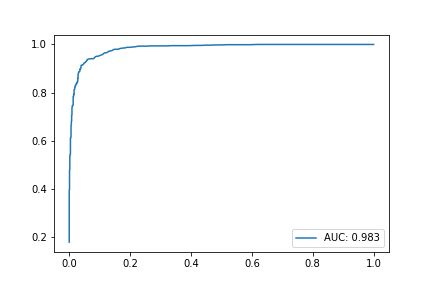
\includegraphics[width = \textwidth]{figures/ROC.png}
		\caption[Example for an ROC curve]{An Example for an ROC curve. It was plotted from a generated dataset with 1000 positive and negative entries respectively, being "scored" using a log normal distribution with different expected values. Calculations were done by the \texttt{pseudoROC} function as described in~\ref{lab:matmet:pseudoROC}.}
		\label{fig:roc_example}
	\end{figure}
	\renewcommand{\baselinestretch}{1}\\
	When dealing with the problem of rating PSMs however, there is no way of knowing the ground truth and thus precisely estimating a classifiers performance. Instead, the total number of PSMs that are estimated to be correct when accepting a certain q-value are plotted against that q-value~\cite{Kll2007, Granholm2012}. The graphs shape resembles that of an ROC curve, and is thus called pseudo ROC. However, there are significant differences and neither the number of accepted PSMs nor the q-value are the same as their ROC counterparts: The q-value of a certain PSM, being related to the FDR, is the (estimated!) portion of wrongly accepted PSMs out of every positively classified PSM, when using the PSMs score as threshold. The false positive rate on the other hand would be the percentage of wrongly accepted PSMs out of every wrong PSM in the whole dataset. With the confusion matrix notation from~\citet{Fawcett2006}, this can be written as:\\
	\begin{equation}
		FDR = \frac{FP}{Y};~~~ FPR = \frac{FP}{n}
	\end{equation}
	With this notation, the true positive rate (TPR) is $\frac{TP}{p}$ and the total number of accepted PSMs is $Y$. From this, a completely different scale arises (since $Y \in \mathbb{N}$ and TPR $\in [0,1]$). The AUC, which is still used as a metric, thus does not range from 0 to 1 and does not represent a probability, but can only be used as a relative score.\\
	ROC curves improve when the data contains more examples with features clearly indicating the negative class membership to the classifier, because the FPR of all other examples decreases. Since pseudo ROCs are plotted only for q-values regarded interesting, often in $[0,0.05]$, they are insensitive to such changes in the data. This allows including lower-scoring PSMs in the dataset~(like is done in this thesis) without diluting the evaluation. Examples for pseudo ROCs are shown in figure~\ref{fig:pseudo_roc_example}.
	\renewcommand{\baselinestretch}{0.9}
	\begin{figure}
		\normalsize
		\centering
		\begin{subfigure}{0.49\textwidth}
			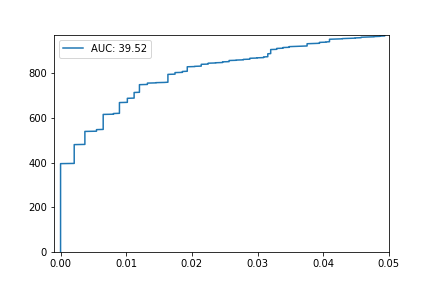
\includegraphics[width = \textwidth]{figures/pseudo_ROC_generated_dataset.png}
			\caption{This pseudo ROC was generated from the same generated dataset as was used for the ROC curve in~\ref{fig:roc_example}.}
		\end{subfigure}
		\hfill
		\begin{subfigure}{0.49\textwidth}
			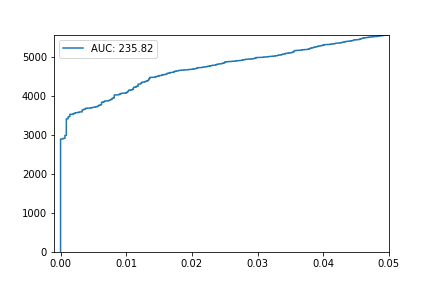
\includegraphics[width = \textwidth]{figures/pseudo_ROC_slow.png}
			\caption{This pseudo ROC is generated from the realistic dataset described in~\ref{lab:matmet:dataset}, using the given NuXL-score.}
		\end{subfigure}
		\caption[Examples for pseudo ROC curves]{Examples for pseudo ROC curves, plotted using the function \texttt{pseudoROC} as described in~\ref{lab:matmet:pseudoROC}.}
		\label{fig:pseudo_roc_example}
	\end{figure}
	\renewcommand{\baselinestretch}{1}